%-----------Entregables  
\newpage
\section*{Entregables}

\subsection*{Cálculo del Error Cuadrático Medio (ECM)}
\noindent El error cuadr\'atico medio es una m\'etrica com\'unmente utilizada para evaluar la 
diferencia entre valores predichos y valores reales. La f\'ormula del error cuadr\'atico es:

$$ ECM = \frac{1}{N} \sum_{i = 1}^{N}(x_i-\hat{x}_i)^2 $$

donde 

\begin{itemize}
  \item N es el número total de muestras
  \item \(x_i\) es el valor real de \textit{sampleRTT} en la i-\'esima medici\'on
  \item \(\hat{x}_i\) es el valor estimado de \textit{estimatedRTT} en la i-\'esima medici\'on
\end{itemize}

\noindent Este valor se utiliza para comparar los diferentes valores de \( \alpha \) en el proceso de estimación.

\subsection*{Implementación de la Estimación de RTT}
\noindent Para este análisis, se emplea el algoritmo de Jacobson para estimar el \( \text{EstimatedRTT} \) 
y el \( \text{RTO} \) a partir de las muestras de \( \text{SampleRTT} \). Se emplean tres valores 
diferentes de \( \alpha \) para estudiar su influencia en el cálculo del \( \text{EstimatedRTT} \),
a saber:
\begin{itemize}
    \item \( \alpha = \frac{1}{8} \) (valor por defecto)
    \item \( \alpha_1 = \frac{1}{4} \)
    \item \( \alpha_2 = \frac{1}{16} \)
\end{itemize}

\subsection*{Análisis de Resultados}
\noindent Se realizaron tres simulaciones para cada valor de \( \alpha \), y se calcularon los valores 
de \( \text{SampleRTT} \), \( \text{EstimatedRTT} \) y \( \text{RTO} \) para cada medición. A 
continuación, se presenta el error cuadrático medio (ECM) para cada uno de los valores de \( \alpha \)

\begin{equation}
  \text{MSE}(\alpha) = \frac{1}{n} \sum_{i=1}^{n} ( \text{SampleRTT}_i - \text{EstimatedRTT}_i )^2
\end{equation}

\subsection*{Gráficas de la Estimación de RTT}
\noindent A continuación se presentan las gráficas de los tres procesos: \( \text{SampleRTT} \), 
\( \text{EstimatedRTT} \) y \( \text{TimeoutInterval} \), para cada valor de \( \alpha \) 
seleccionado. El eje \( x \) representa el número de la medición (número de vuelta), 
mientras que el eje \( y \) muestra los valores de los procesos.

\begin{figure}[H]
    \centering
    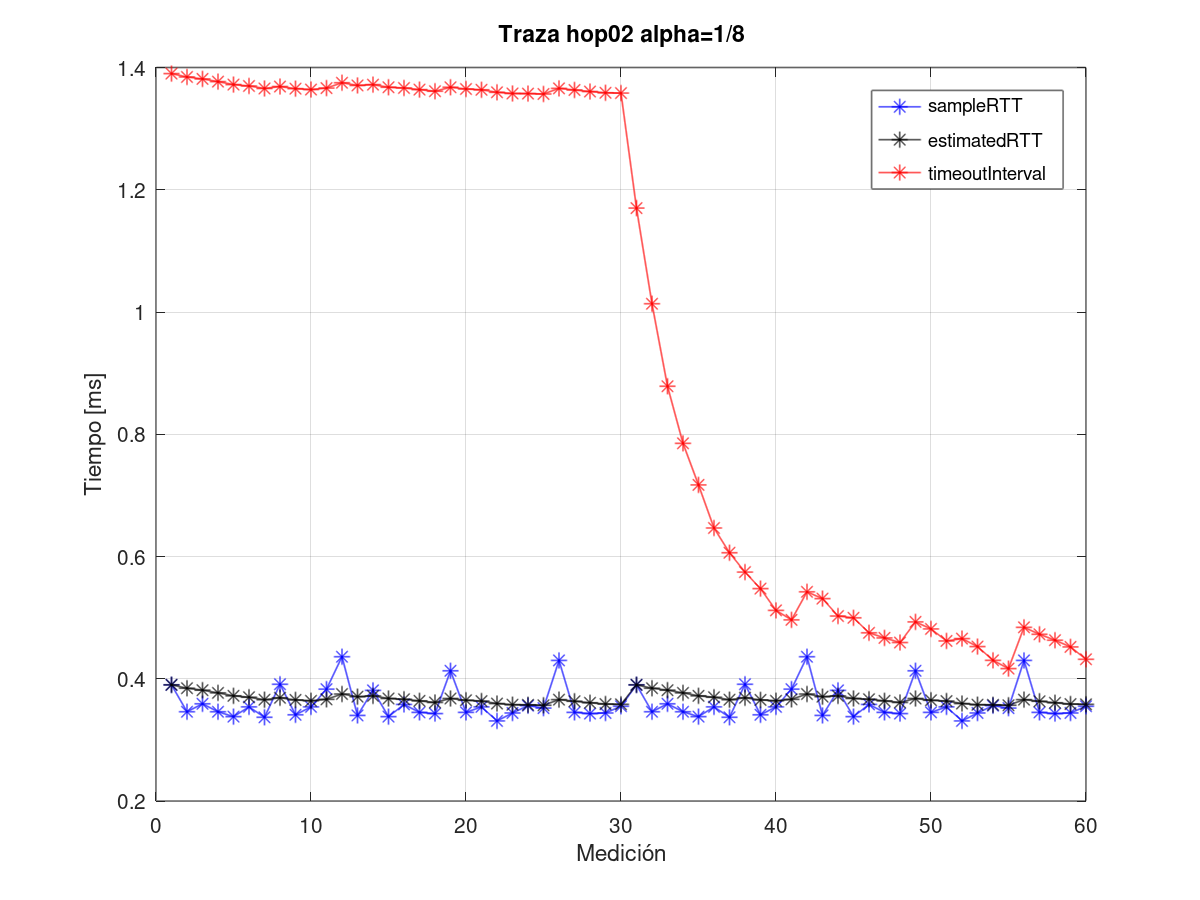
\includegraphics[width=0.75\textwidth]{img/alpha18/trazahop02.png}
    \caption{Gráfica de SampleRTT, EstimatedRTT y TimeoutInterval con \( \alpha = \frac{1}{8} \)
    de la muestra hop02}

    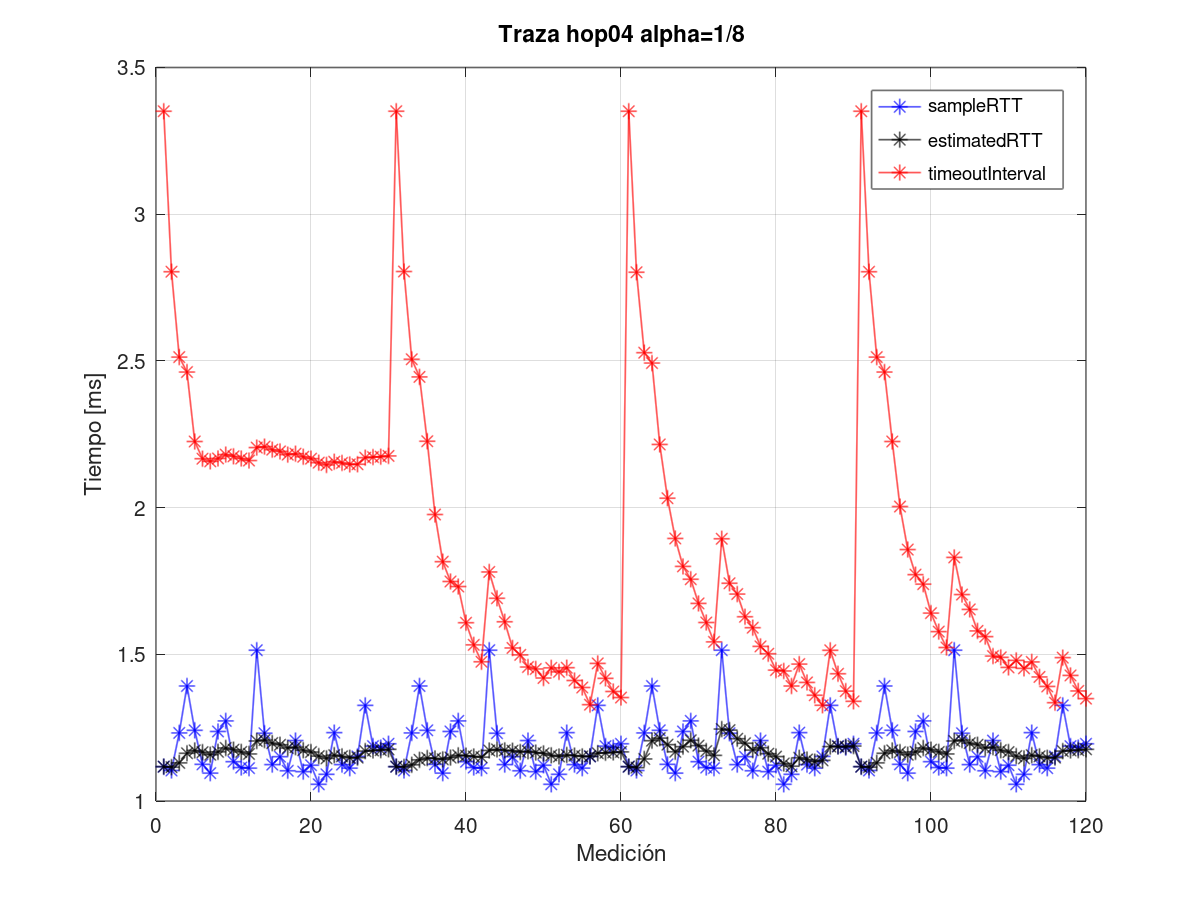
\includegraphics[width=0.75\textwidth]{img/alpha18/trazaHop04.png}
    \caption{Gráfica de SampleRTT, EstimatedRTT y TimeoutInterval con \( \alpha = \frac{1}{8} \)
    de la muestra hop04}
    \label{fig:alpha_default_p1}
\end{figure}
\newpage
\begin{figure}[H]
  \centering
  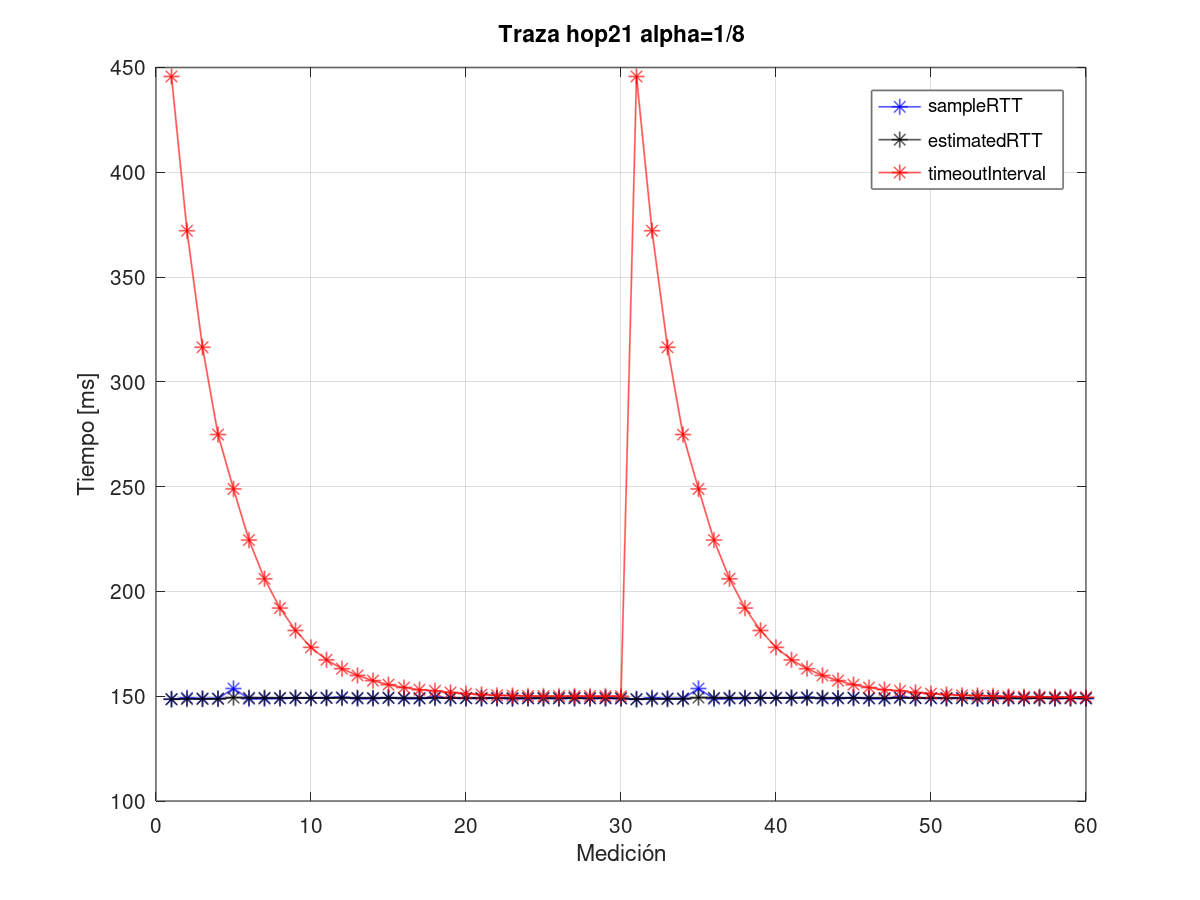
\includegraphics[width=0.75\textwidth]{img/alpha18/trazaHop21.png}
  \caption{Gráfica de SampleRTT, EstimatedRTT y TimeoutInterval con \( \alpha = \frac{1}{8} \)
  de la muestra hop21}

  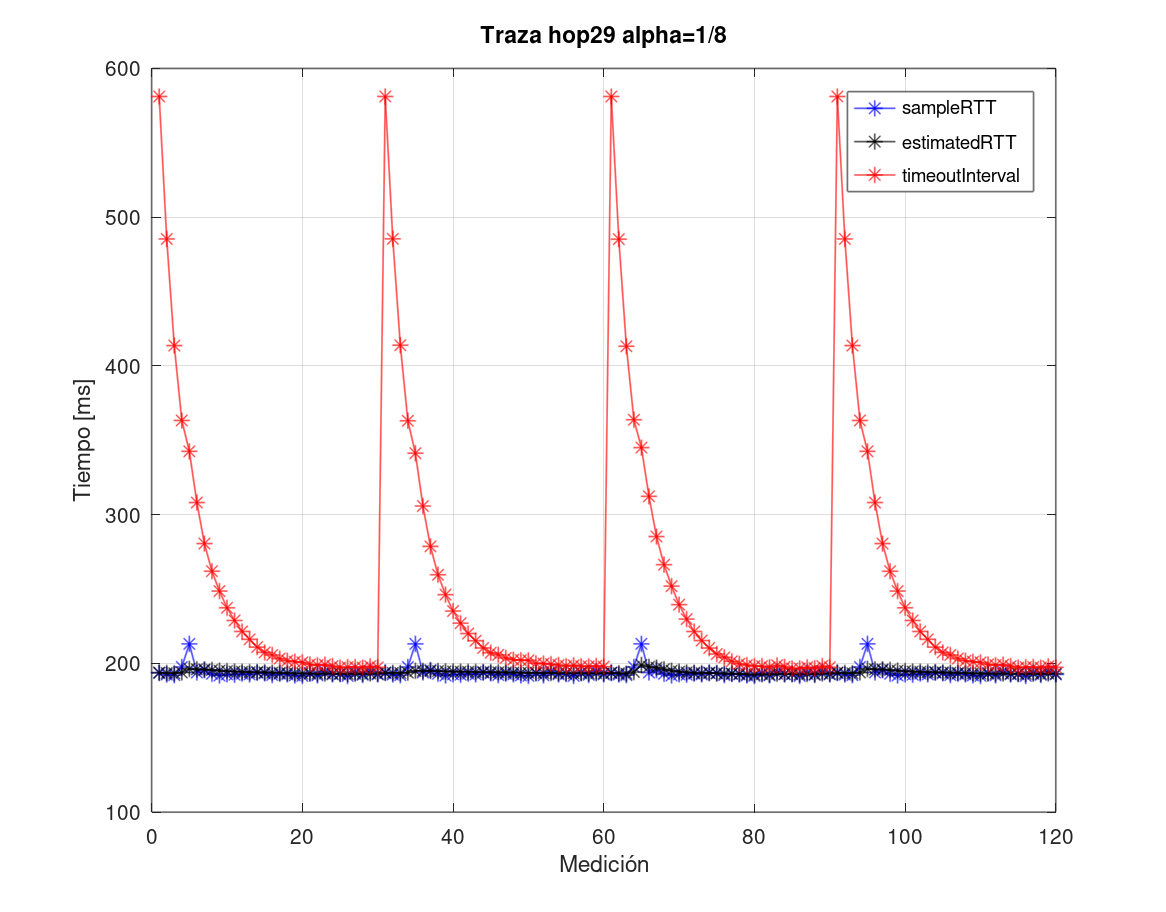
\includegraphics[width=0.75\textwidth]{img/alpha18/trazaHop29.png}
  \caption{Gráfica de SampleRTT, EstimatedRTT y TimeoutInterval con \( \alpha = \frac{1}{8} \)
  de la muestra hop29}
  \label{fig:alpha_default_p2}
\end{figure}

\begin{figure}[H]
    \centering
    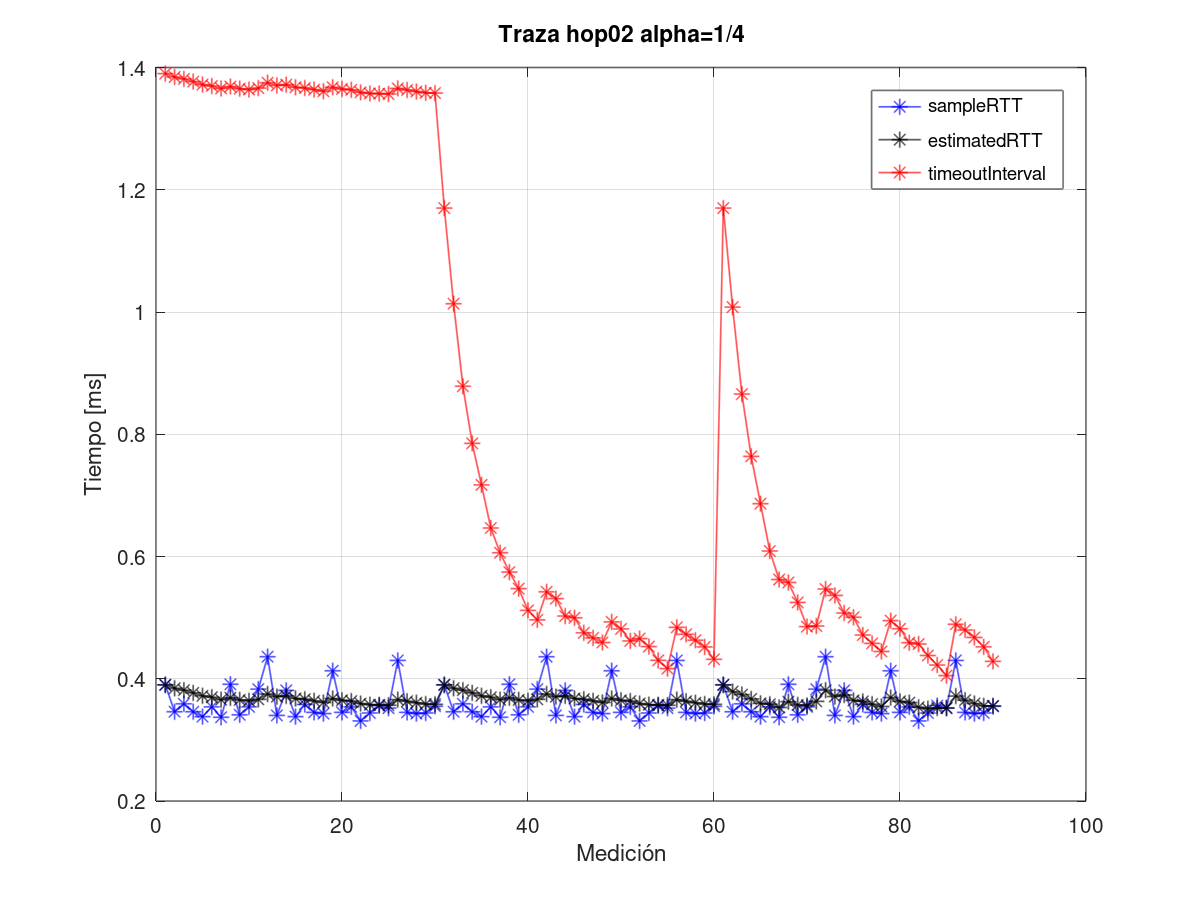
\includegraphics[width=0.75\textwidth]{img/alpha14/trazaHop02.png}
    \caption{Gráfica de SampleRTT, EstimatedRTT y TimeoutInterval con \( \alpha = \frac{1}{4} \)
    de la muestra hop02}

    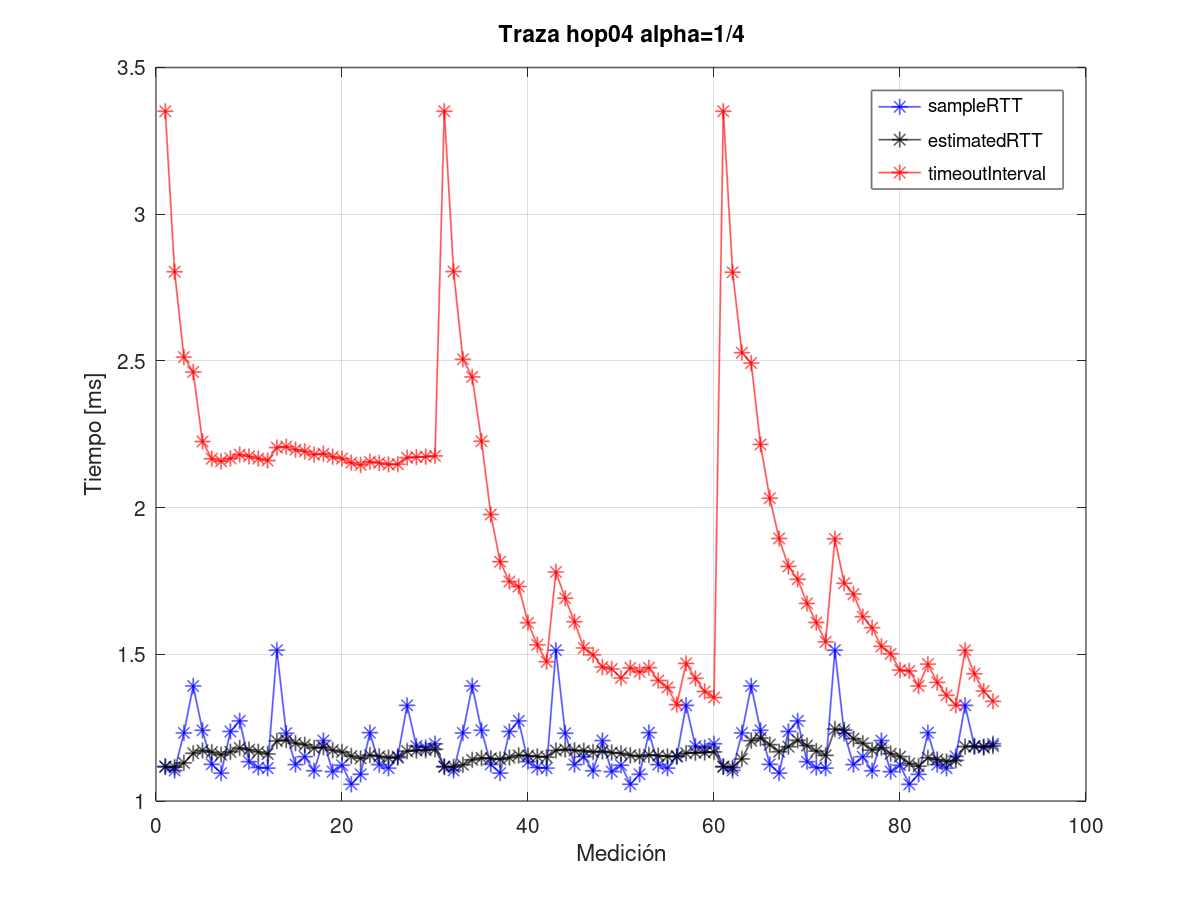
\includegraphics[width=0.75\textwidth]{img/alpha14/trazaHop04.png}
    \caption{Gráfica de SampleRTT, EstimatedRTT y TimeoutInterval con \( \alpha = \frac{1}{4} \)
    de la muestra hop04}
    \label{fig:alpha1_p1}
\end{figure}
\newpage
\begin{figure}[H]
  \centering
  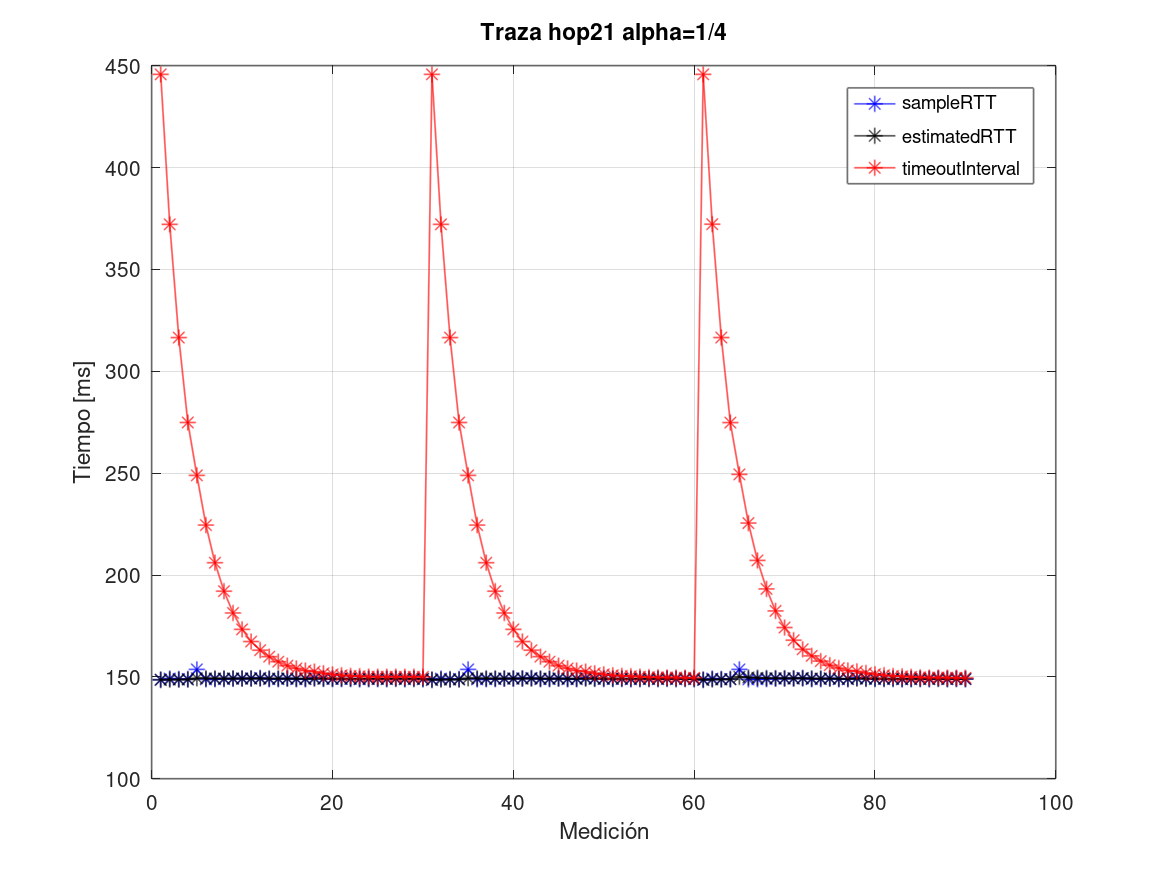
\includegraphics[width=0.75\textwidth]{img/alpha14/trazaHop21.png}
  \caption{Gráfica de SampleRTT, EstimatedRTT y TimeoutInterval con \( \alpha = \frac{1}{4} \)
  de la muestra hop21}

  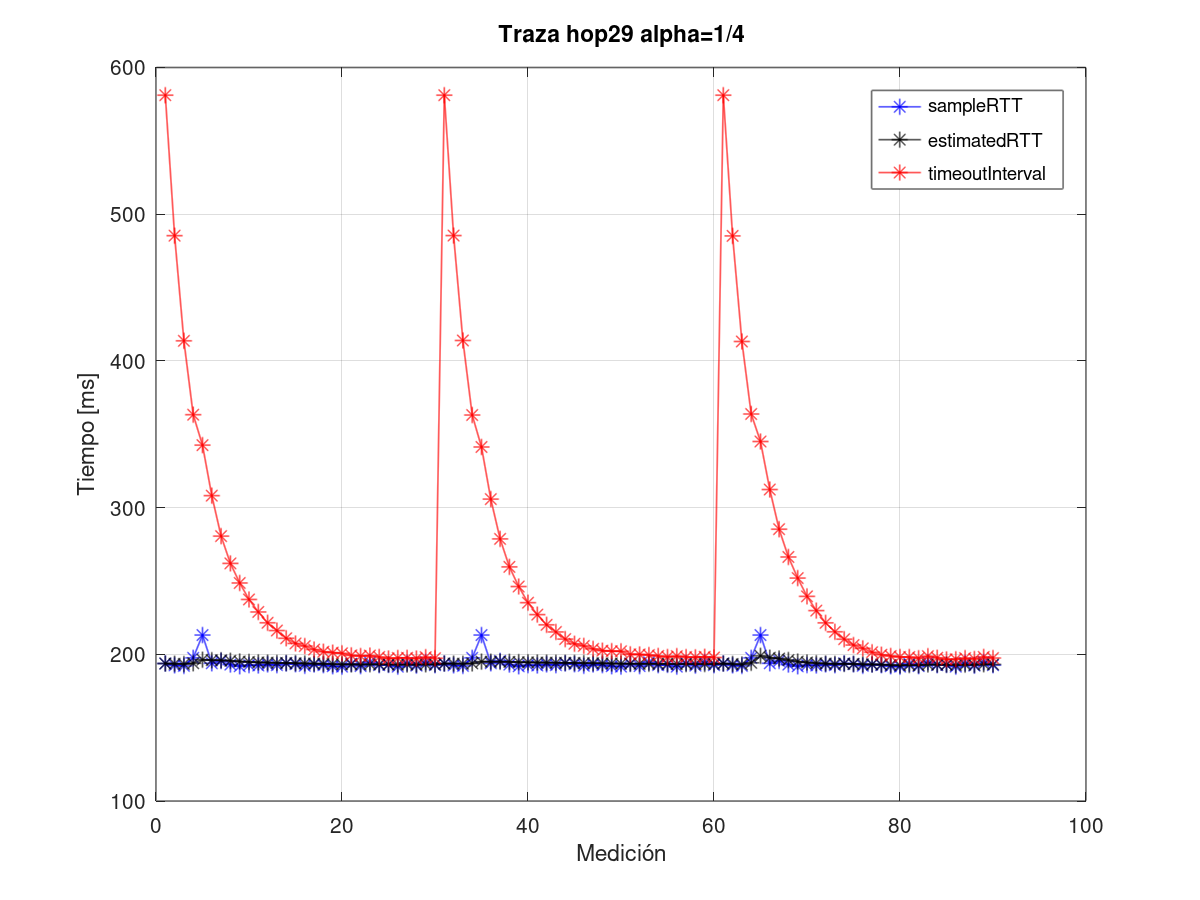
\includegraphics[width=0.75\textwidth]{img/alpha14/trazaHop29.png}
  \caption{Gráfica de SampleRTT, EstimatedRTT y TimeoutInterval con \( \alpha = \frac{1}{4} \)
  de la muestra hop29}
  \label{fig:alpha1_p2}
\end{figure}

\begin{figure}[H]
    \centering
    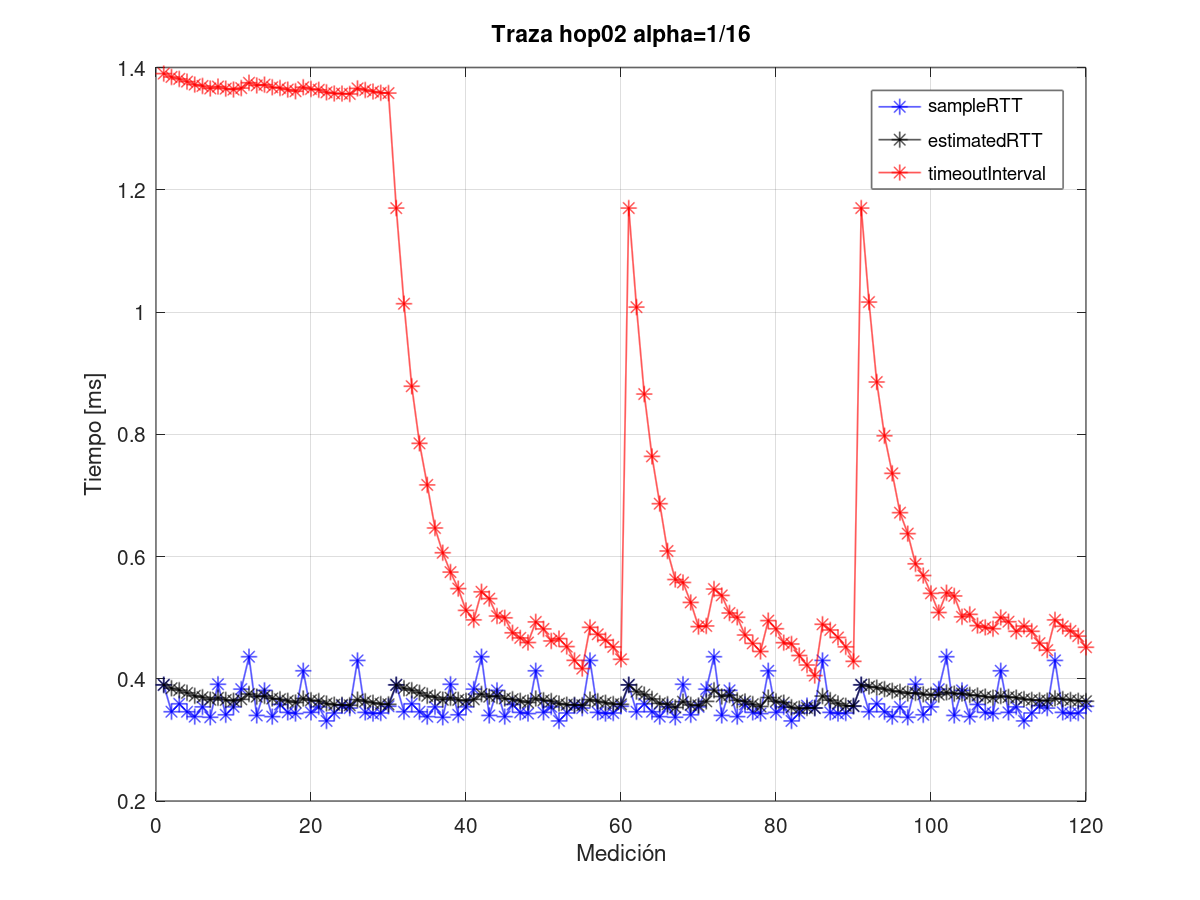
\includegraphics[width=0.75\textwidth]{img/alpha116/trazaHop02.png} 
    \caption{Gráfica de SampleRTT, EstimatedRTT y TimeoutInterval con \( \alpha = \frac{1}{16} \)
    de la muestra hop02}

    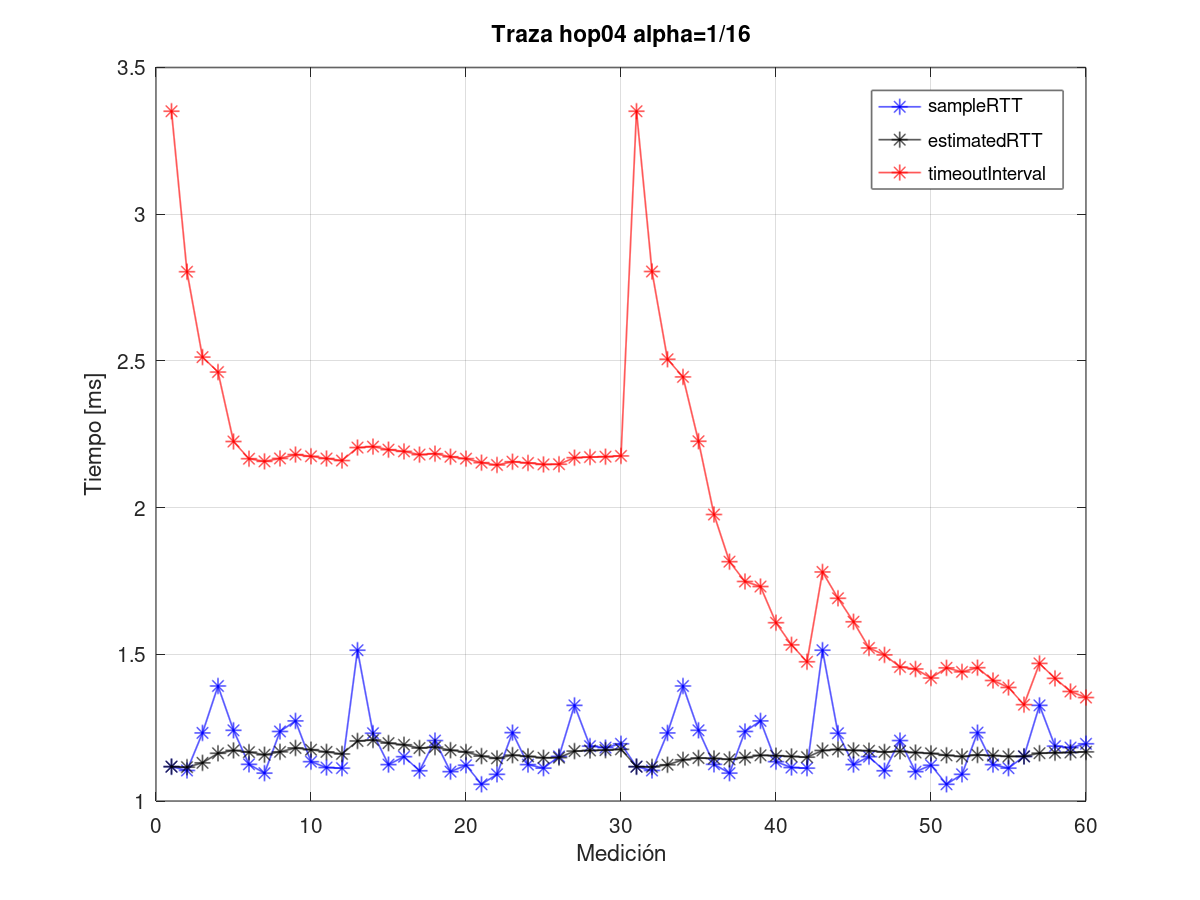
\includegraphics[width=0.75\textwidth]{img/alpha116/trazaHop04.png} 
    \caption{Gráfica de SampleRTT, EstimatedRTT y TimeoutInterval con \( \alpha = \frac{1}{16} \)
    de la muestra hop04}
    \label{fig:alpha2_p1}
\end{figure}
\newpage
\begin{figure}[H]
  \centering
  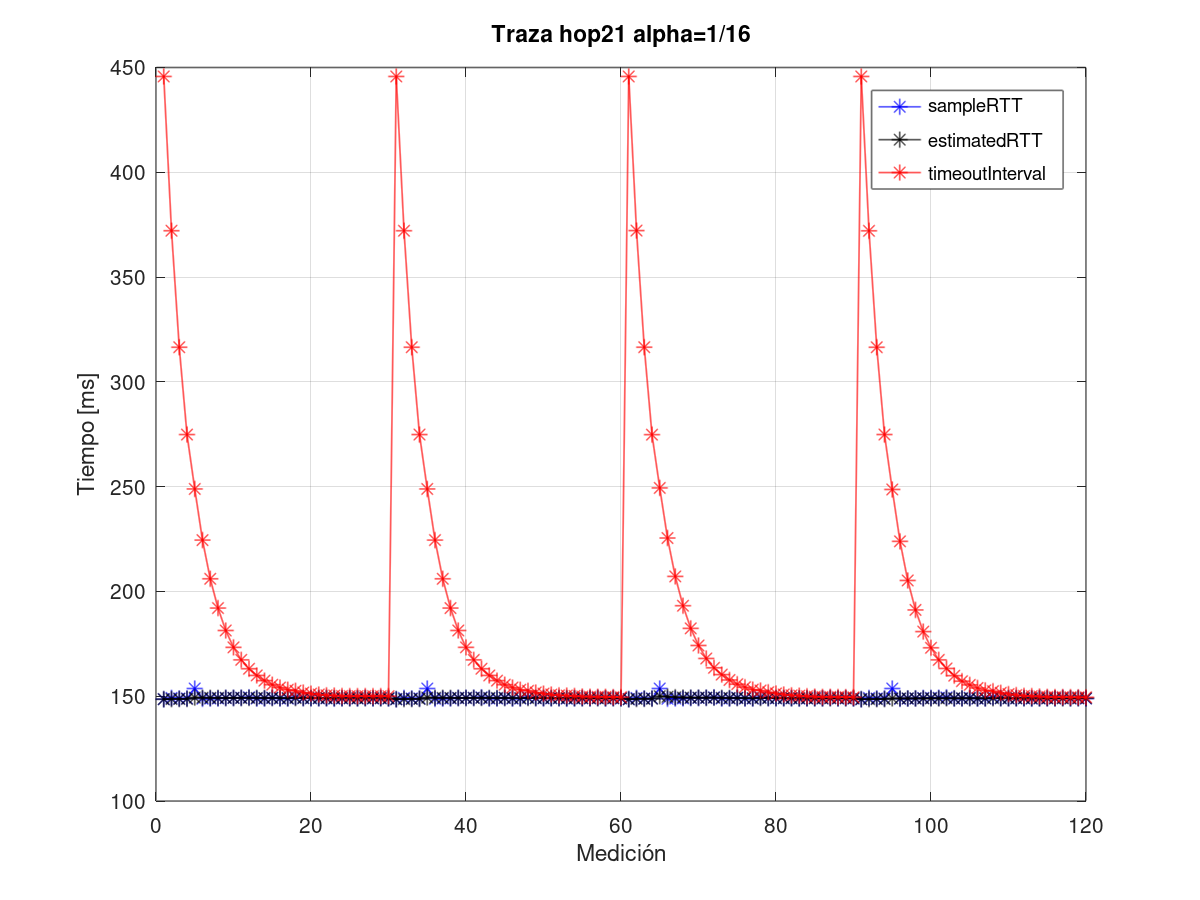
\includegraphics[width=0.75\textwidth]{img/alpha116/trazaHop21.png} 
  \caption{Gráfica de SampleRTT, EstimatedRTT y TimeoutInterval con \( \alpha = \frac{1}{16} \)
  de la muestra hop21}

  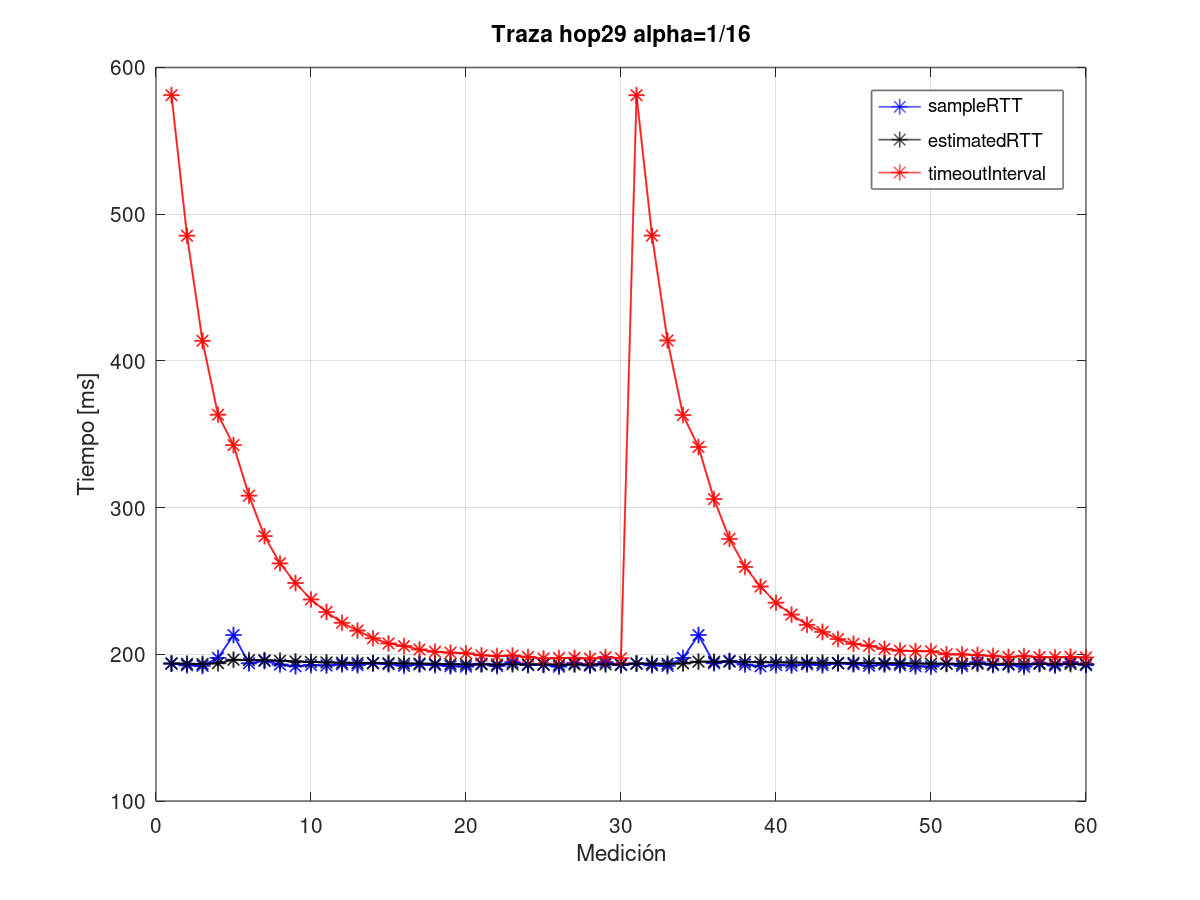
\includegraphics[width=0.75\textwidth]{img/alpha116/trazaHop29.png} 
  \caption{Gráfica de SampleRTT, EstimatedRTT y TimeoutInterval con \( \alpha = \frac{1}{16} \)
  de la muestra hop29}
  \label{fig:alpha2_p2}
\end{figure}

\subsection*{Discusión y Conclusiones}
\noindent A partir de las gráficas obtenidas y el análisis de los errores cuadráticos medios (ECM) 
para cada valor de \( \alpha \), podemos concluir que:

\begin{itemize}
    \item El valor de \( \alpha = \frac{1}{8} \) (por defecto) produce una estimación bastante precisa,
    con un ECM moderado.
    \item Un valor mayor de \( \alpha \), como \( \alpha_1 = \frac{1}{4} \), aumenta la sensibilidad
    del algoritmo, lo que puede generar un mayor error en entornos con fluctuaciones rápidas en
    \( \text{SampleRTT} \).
    \item Un valor menor de \( \alpha \), como \( \alpha_2 = \frac{1}{16} \), reduce la sensibilidad
    del algoritmo, lo que puede ser útil en entornos estables, pero puede no reaccionar rápidamente 
    ante cambios importantes en el RTT.
\end{itemize}


